% -*- TeX-engine: xetex -*-

\documentclass[xetex,aspectratio=169,14pt,hyperref={pdfpagelabels=true,pdflang={en-GB}}]{beamer}

\usepackage[sci,noslidestrathidentity]{strathclyde}
\strathsetidentity{Department of}{Computer \& Information Sciences}

\usepackage{lmodern}
\usepackage{subscript}
\usepackage{url}
\usepackage{pifont}
\usepackage{csquotes}
\usepackage{mathpartir}
\usepackage{stmaryrd}
\usepackage{multirow}
\usepackage{euler}
\usepackage[normalem]{ulem}

% 2013-09-08 SU adding xetex specifics
% http://www.woggie.net/2008/07/16/beamer-pdftex-and-xetex/
\usepackage{xltxtra}

% 2013-09-08 SU http://robjhyndman.com/hyndsight/xelatex/
\defaultfontfeatures{Ligatures=TeX}

% 2015-12-09 SU table beautified
\renewcommand{\arraystretch}{1.2}
\usepackage{booktabs}

%MGK compatibility
\newcommand{\hh}[1]
  {\medskip\textbf{\large #1}}
\newcommand{\pdu}[3]
  {#1\rightarrow #2 : &\ & \makebox[70mm][l]{$#3$}}



\setlength{\marginparwidth}{2cm}
\usepackage{todonotes}%[disable]
\let\OldTodo\todo
\renewcommand{\todo}{\OldTodo[inline]}%
\newcommand{\todolater}[1]{}% Things to do for next year


\DeclareTextCommandDefault{\nobreakspace}{\leavevmode\nobreak\ }
\usepackage{rotating}

\usepackage{pdfcomment}% To add alt text for images using \pdftooltip{}

\usepackage{appendixnumberbeamer}

\newcommand{\messageframe}[1]{\begin{frame}\begin{center}\Huge #1\end{center}\end{frame}}
\newcommand{\sechead}[1]{{\bf #1} \\}
\newcommand{\examplehead}[1]{{\bf Example:} {\it\textcolor{red!90}{#1}} \\}
\newcommand{\eqnote}[1]{\hspace{3cm}\textit{#1}}
\newcommand{\sidenote}[1]{\qquad {\footnotesize \textcolor{black!60}{(#1)}}}
\newcommand{\sem}[1]{\llbracket #1 \rrbracket}
\newcommand{\true}{\mathsf{T}}
\newcommand{\false}{\mathsf{F}}

\def\strikeafter<#1>#2{\temporal<#1>{#2}{\sout{#2}}{\sout{#2}}}


%\newcommand{\rhighlight}{\textcolor{titlered}}
\newcommand{\rhighlight}{\textbf}
\newcommand{\highlight}{\textbf}

% \setmainfont{Linux Biolinum O}
\setmainfont{LinBiolinum}[
Path=,
UprightFont = *_R.otf ,
BoldFont = *_RB.otf ,
ItalicFont = *_RI.otf
]

\setbeamertemplate{navigation symbols}{}
%\usecolortheme[rgb={0.8,0,0}]{structure}
\usefonttheme{serif}
\usefonttheme{structurebold}
\setbeamercolor{description item}{fg=black}


\author[Atkey]{Dr.~Robert Atkey}
\institute[Strathclyde]{Computer \& Information Sciences}
\date[]{}

\newcommand{\weeksection}[1]{%
  \section{\thetitle{}, Part~\thesection : #1}
  \begin{frame}
    \begin{center}
      \textcolor{black!60}{\thetitle{}, Part \thesection}\\
      {\Huge #1}
    \end{center}
  \end{frame}}

\newcommand{\weektitle}[2]{\def\thetitle{#2}
\title[CS208 - Topic #1]{CS208 (Semester 1) Topic #1 : #2}}

\newcommand{\assigned}{:}

\newcommand{\forcedto}{\assigned_f}
\newcommand{\decideto}{\assigned_d}


\weektitle{0}{Propositional Logic}

\begin{document}

\frame{\titlepage}

\weeksection{Syntax}

\begin{frame}
  {Atomic Statements}

  \emph{Propositional Logic} is concerned with statements that make
  assertions (about the world, or about some ``situation''):
  \begin{enumerate}
  \item ``It is raining''
  \item ``I am in Glasgow''
  \item ``Version 2.1 of \emph{libfoo} is installed''
  \item ``The number in cell $(3,3)$ is $7$''
  \end{enumerate}
  usually, we abbreviate these: $R$, $G$, $\mathit{foo}_{2.1}$, $C^{3,3}_7$

  \medskip

  These are called \emph{atomic statements} or \emph{atoms}.
\end{frame}

\begin{frame}
  {Compound Statements}

  \begin{enumerate}
  \item $R \to G$ \\ \qquad{\it if it is raining, I am in Glasgow} \\
    \medskip
  \item $\lnot R \to \lnot G$ \\ \qquad{\it if it is not raining, then I am not in Glasgow} \\
    \medskip
  \item $\lnot\mathit{foo}_{2.1} \lor \lnot\mathit{foo}_{2.0}$\\
    \qquad {\it
      either version 2.1 or 2.0 of $\mathit{libfoo}$ is not installed} \\
    \medskip
  \item $C^{3,3}_7 \land C^{3,4}_8$\\
    \qquad {\it cell $(3,3)$ contains $7$, and cell $(3,4)$ contains $8$}
  \end{enumerate}
\end{frame}

\begin{frame}
  {Formulas}

  ... are built from \emph{atomic propositions} $A, B, C, \cdots$, and
  the \emph{connectives} $\land$ (``and''), $\lor$ (``or''), $\lnot$
  (``not''), and $\to$ (``implies'').

  \medskip

  As a grammar:
  \begin{displaymath}
    P, Q ::= A \mid P \land Q \mid P \lor Q \mid \lnot P \mid P \to Q
  \end{displaymath}
  where $A$ stands for any atomic proposition.

  \bigskip

  Typically, formulas are written done in a ``linear'' notation, like
  in algebra. This is because it is more compact...

\end{frame}

\begin{frame}
  \centering
  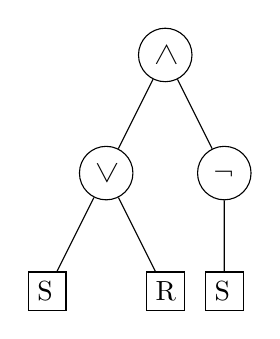
\begin{tikzpicture}
    \tikzstyle{op}=[draw,circle,text width=0.7em,text height=0.7em]
    \tikzstyle{atom}=[draw,rectangle,text width=0.7em,text height=0.7em]
    \path
    node[op] {$\land$}
    child {
      node[op] {$\lor$}
      child { node[atom] {S} }
      child { node[atom] {R} }
    }
    child {
      node[op] {$\lnot$}
      child { node[atom] {S} }
    };
  \end{tikzpicture}

  \pause
  \begin{displaymath}
    (S \lor R) \land \lnot S
  \end{displaymath}
\end{frame}

\begin{frame}
  \centering
  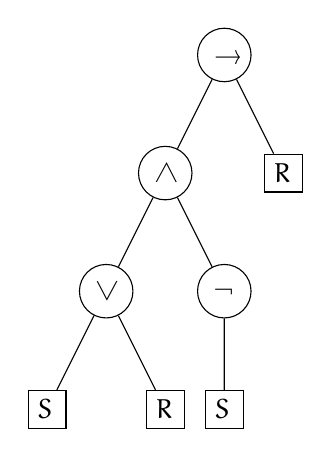
\begin{tikzpicture}
    \tikzstyle{op}=[draw,circle,text width=0.7em,text height=0.7em]
    \tikzstyle{atom}=[draw,rectangle,text width=0.7em,text height=0.7em]
    \path
    node[op] {$\to$}
    child {
      node[op] {$\land$}
      child {
        node[op] {$\lor$}
        child { node[atom] {$S$} }
        child { node[atom] {$R$} }
      }
      child {
        node[op] {$\lnot$}
        child { node[atom] {$S$} }
      }
    }
    child {
      node[atom] {$R$}
    };
  \end{tikzpicture}

  \pause
  \begin{displaymath}
    ((S \lor R) \land \lnot S) \to R
  \end{displaymath}
\end{frame}


\begin{frame}
  {Ambiguity}

  For compactness, we write out formulas ``linearly'':
  \begin{displaymath}
    \begin{array}{ll}
      (S \lor R) \land \lnot S &
      ((S \lor R) \land \lnot S) \to R
    \end{array}
  \end{displaymath}

  \medskip

  However, this is ambiguous. What tree does this represent?
  \begin{displaymath}
    S \lor R \land \lnot S \to R
  \end{displaymath}
  we disambiguate with parentheses:
  \begin{displaymath}
    ((S \lor R) \land \lnot S) \to R
  \end{displaymath}
  Could put parentheses around every connective, but this is messy.
\end{frame}

\begin{frame}
  {Disambiguation}
  \begin{enumerate}
  \item Runs of $\land$, $\lor$, $\to$ associate to the right:
    \begin{displaymath}
      P_1 \land P_2 \land P_3 \land P_4 \quad \textrm{ is same as }\quad P_1 \land (P_2 \land (P_3 \land P_4))
    \end{displaymath}
  \item For any binary connective inside another, require parentheses:
    \begin{displaymath}
      \begin{array}{ll@{\hspace{3em}}ll}
        (P_1 \lor P_2) \land P_3&\textrm{good} &
        P_1 \lor P_2 \land P_3&\textrm{bad}
      \end{array}
    \end{displaymath}
  \item For a binary connective under a $\lnot$, require parentheses:
    \begin{displaymath}
        \lnot P \land Q \quad \textrm{ is not the same as } \quad \lnot (P \land Q)
    \end{displaymath}
  \item We don't put parentheses around a $\lnot$:
    \begin{displaymath}
      \begin{array}{ll@{\hspace{3em}}ll}
        \lnot (P \land Q) &\textrm{good} &
        (\lnot (P \land Q)) &\textrm{bad}
      \end{array}
    \end{displaymath}
  \end{enumerate}

\end{frame}

\def\hiddenuntil<#1>#2{{\temporal<#1>{\color{black!0}}{\color{black}}{\color{black}} #2}}

\begin{frame}
  \frametitle{Decomposing Formulas}

  Split into: \emph{a)} toplevel connective;\emph{b)} immediate subformulas

  \bigskip

  \begin{tabular}{l|l|l}
    Formula & Connective & Subformulas\\
    \hline
    $A \land B$ & \hiddenuntil<2>{$\land$} & \hiddenuntil<2>{$A$ and $B$} \\
    $A \land B \land C$ & \hiddenuntil<3>{$\land$} & \hiddenuntil<3>{$A$ and $B \land C$} \\
    $\lnot(A \land B)$ & \hiddenuntil<4>{$\lnot$} & \hiddenuntil<4>{$A \land B$} \\
    $A \to B \to C \to D$ & \hiddenuntil<5>{$\to$} & \hiddenuntil<5>{$A$ and $B \to C \to D$} \\
    $B \to C \to D$ & \hiddenuntil<6>{$\to$} & \hiddenuntil<6>{$B$ and $C \to D$} \\
  \end{tabular}
\end{frame}
\begin{frame}
  \frametitle{Decomposing Formulas}

  Split into: \emph{a)} toplevel connective;\emph{b)} immediate subformulas

  \begin{tabular}{l|l|l}
    Formula & Connective & Subformulas\\
    \hline
    $(A \land B) \to (A \lor B)$ & \hiddenuntil<2>{$\to$} & \hiddenuntil<2>{$(A \land B)$ and $(A \lor B)$} \\
    $(A \land B) \lor (B \land C)$ & \hiddenuntil<3>{$\lor$} & \hiddenuntil<3>{$(A \land B)$ and $(B \land C)$} \\
    $A \lor B \lor C$ & \hiddenuntil<4>{$\lor$} & \hiddenuntil<4>{$A$ and $B \lor C$} \\
    $A \lor B \land C$ & \hiddenuntil<5>{?} & \hiddenuntil<5>{?}
  \end{tabular}

  \bigskip

  \hiddenuntil<5>{Last one is ambiguous! $A \lor (B \land C)$ or $(A \lor B) \land C$?}
\end{frame}

\begin{frame}
  {Summary}

  Propositional Logic formulas comprise:
  \begin{enumerate}
  \item Atomic propositions
  \item Compound formulas built from $\land$, $\lor$, $\to$, $\lnot$
  \end{enumerate}

  \bigskip

  Formulas are ``really'' trees, but we write them linearly.

  \bigskip

  We use parentheses to disambiguate.
\end{frame}

\weeksection{Semantics}

\begin{frame}
  {Truth Values}

  We define the semantics of formulas in terms of \rhighlight{truth values}:

  \begin{itemize}
  \item $\true$ --- meaning ``true'', also written $1$, $\top$, $\mathsf{t}$, $\mathsf{true}$;
  \item $\false$ --- meaning ``false'', also written $0$, $\bot$, $\mathsf{f}$, $\mathsf{false}$.
  \end{itemize}

  \bigskip
  \pause

  \begin{itemize}
  \item Other collections of truth values are possible \\
    \qquad\textcolor{black!60}{(e.g., ``unknown'', or values between $0$ and $1$)}
  \item The truth values mean whatever we want them to mean:
    \begin{itemize}
    \item Current or no current on a wire
    \item Package is installed or not installed
    \item Grid cell is filled or not
    \end{itemize}
  \end{itemize}
\end{frame}

\begin{frame}
  {Meaning is Compositional}

  \vspace{0.75em}

  \quad \rhighlight{The Meaning of a Formula is Defined In Terms of its Parts}

  \pause
  \bigskip

  To work out the meaning of $P \land Q$:
  \begin{enumerate}
  \item Work out the meaning of $P$
  \item Work out the meaning of $Q$
  \item Combine using the meaning of $\land$ \textcolor{black!60}{and similar for $\to$, $\lor$, $\lnot$.}
  \end{enumerate}


  \pause
  \bigskip

  This recipe leaves us to determine:
  \begin{enumerate}
  \item What is the meaning of an atom $A$?
  \item What is the meaning of $\to$, $\land$, $\lor$, $\lnot$?
  \end{enumerate}
\end{frame}

\begin{frame}
  {Valuations}

  An assignment of truth values to atomic propositions is called a
  \rhighlight{valuation}. We use the letter $v$ to stand for
  valuations.

  \medskip

  For an atom $A$, we write $v(A)$ for the value assigned
  to $A$ by $v$.

  \bigskip
  \pause

  \textbf{Example}
  \begin{displaymath}
    v = \{ A \assigned \true, B \assigned \false, C \assigned \true \}
  \end{displaymath}
  So: $\begin{array}[t]{l@{\hspace{0.2em}}c@{\hspace{0.2em}}c}
         v(A) &=& \true \\
         v(B) &=& \false \\
         v(C) &=& \true
       \end{array}$

\end{frame}

\begin{frame}
  {Example Valuations}

  \begin{enumerate}
  \item $v = \{ S \assigned \true, R \assigned \false \}$ \\
    \quad \textcolor{black!60}{``It is sunny $(v(S) = \true\hspace{0.1em})$. It is not raining $(v(R) = \false\hspace{0.1em})$''}
  \item $v = \{ S \assigned \false, R \assigned \true \}$ \\
    \quad \textcolor{black!60}{``It is not sunny $(v(S) = \false\hspace{0.1em})$. It is raining $(v(R) = \true\hspace{0.1em})$''}
  \item $v = \{ S \assigned \true, R \assigned \true \}$ \\
    \quad \textcolor{black!60}{``It is sunny $(v(S) = \true\hspace{0.1em})$. It is raining $(v(R) = \true\hspace{0.1em})$''}
  \end{enumerate}

  \pause
  \bigskip

  \textcolor{black!60}{Intuition: }Valuations describe ``states of the world''
\end{frame}

\begin{frame}
  {Notes on Writing Valuations}

  \begin{enumerate}
  \item Two valuations are equal if they assign the same truth values
    to the same atoms.\\
    \quad \textcolor{black!60}{Order of writing them down doesn't matter.}
  \item Each atom can only be assigned one truth value.
  \item Every relevant atom must be assigned some truth value.
  \end{enumerate}

\end{frame}

\begin{frame}
  {Semantics of the Connectives}

  \begin{center}
    \begin{tabular}{ll}
      Formula & {\it is true when ...} \\
      \hline
      $P \land Q$ & both $P$ and $Q$ are true\\
      $P \lor Q$ & at least one of $P$ or $Q$ is true\\
      $\lnot P$ & $P$ isn't true\\
      $P \to Q$ & if $P$ is true, then $Q$ is true\\
      & {\it otherwise it is false.}
    \end{tabular}
  \end{center}
\end{frame}

\begin{frame}
  {Semantics of the Connectives I}

  \begin{mathpar}
    \begin{array}{cc|c}
      P&Q&P \land Q \\
      \hline
      \false&\false&\false\\
      \false&\true&\false\\
      \true&\false&\false\\
      \true&\true&\true\\
    \end{array}

    \begin{array}{cc|c}
      P&Q&P \lor Q \\
      \hline
      \false&\false&\false\\
      \false&\true&\true\\
      \true&\false&\true\\
      \true&\true&\true\\
    \end{array}
  \end{mathpar}
\end{frame}

\begin{frame}
  {Semantics of the Connectives II}

  \begin{mathpar}
    \begin{array}{c|c}
      P&\lnot P \\
      \hline
      \false&\true \\
      \true&\false
    \end{array}

    \begin{array}{cc|c}
      P&Q&P \to Q \\
      \hline
      \false&\false&\true\\
      \false&\true&\true\\
      \true&\false&\false\\
      \true&\true&\true\\
    \end{array}
  \end{mathpar}

\end{frame}

\begin{frame}
  {Truth Assignment}

  For a formula $P$ and a valuation $v$, we write
  \begin{displaymath}
    \sem{P}v
  \end{displaymath}
  to mean ``the truth value of $P$ at the valuation $v$''.\\
%  \sidenote{The brackets $\sem{\cdot}$ usually mean ``meaning of''.}

  \pause

  \begin{displaymath}
    \begin{array}{lcl}
      \sem{A}v&=&v(A)\\
      \sem{P \land Q}v&=&\sem{P}v \land \sem{Q}v \\
      \sem{P \lor Q}v&=&\sem{P}v \lor \sem{Q}v \\
      \sem{\lnot P}v&=&\lnot \sem{P}v \\
      \sem{P \to Q}v&=&\sem{P}v \to \sem{Q}v \\
    \end{array}
  \end{displaymath}
\end{frame}

\begin{frame}
  {Example}

  $(A \lor B) \land \lnot A$ with the valuation
  $v = \{A \assigned \false, B \assigned \true\}$:

%  FIXME: highlight the bit that changes

  \begin{displaymath}
    \begin{array}{cl}
      ~~~&\sem{(A \lor B) \land \lnot A}v \hspace{3cm}\\
%      \\
      \only<2->{=&\sem{A \lor B}v \land \sem{\lnot A}v} \\
%      \\
      \only<3->{=&(\sem{A}v \lor \sem{B}v) \land \sem{\lnot A}v} \\
%      \\
      \only<4->{=&(\sem{A}v \lor \sem{B}v) \land \lnot \sem{A}v} \\
%      \\
      \only<5->{=&(v(A) \lor v(B)) \land \lnot v(A)} \\
%      \\
      \only<6->{=&(\false \lor \true) \land \lnot \false} \\
%      \\
      \only<7->{=&\true \land \lnot \false} \\
%      \\
      \only<8->{=&\true \land \true}
      \only<9->{=\true}
    \end{array}
  \end{displaymath}
\end{frame}

\begin{frame}
  {Semantics of a Formula}

  For a formula $P$, its \emph{meaning} is the collection of all
  valuations $v$ that make $\sem{P}v = \true$.

  \bigskip

  For example,
  \begin{displaymath}
    \sem{(A \lor B) \land \lnot A} = \left\{
      \begin{array}[t]{@{}l}
        \{A \assigned \false, B \assigned \true\}
      \end{array}\right\}
  \end{displaymath}

  To compute sets of valuations, we will use truth tables.
\end{frame}

\begin{frame}
  {Summary}

  \begin{enumerate}
  \item Semantics defines the \emph{meaning} of formulas.
  \item We use \emph{truth values} $\true$ and $\false$.
  \item A valuation $v$ assigns truth values to atoms.
  \item We extend that assignment to whole formulas: $\sem{P}v$.
  \item The meaning of $P$ is the set of valuations that make it true.
  \end{enumerate}
\end{frame}

\weeksection{Truth Tables, Satisfiability, and Validity}

% \section{Propositional Logic 3 : Truth Tables, Satisfiability and Validity}

% \begin{frame}
%   \begin{center}
%     {\Huge \textcolor{black!60}{Part 3 : }Truth Tables, \\ Satisfiability and Validity}
%   \end{center}
% \end{frame}

\begin{frame}
  \frametitle{Truth table for $(A \lor B) \land \lnot A$}

  Name the parts: $\textcircled{1} = A \lor B$; $\textcircled{2} = \lnot A$

  \begin{center}
    \begin{tabular}{cc||cc|c}
      \multirow{2}{*}{$A$} &
      \multirow{2}{*}{$B$} &
      \textcircled{1} & \textcircled{2} &
      $\text{\textcircled{1}} \land \text{\textcircled{2}}$
      \\
      &&
      $A \lor B$&
      $\lnot A$&
      $(A \lor B) \land \lnot A$
      \\ \hline
      $\false$ & $\false$ & \only<2->{$\false$} & \only<6->{$\true$}  & \only<10->{$\false$} \\
      $\false$ & $\true$  & \only<3->{$\true$}  & \only<7->{$\true$}  & \only<11->{$\true$}  \\
      $\true$  & $\false$ & \only<4->{$\true$}  & \only<8->{$\false$} & \only<12->{$\false$}  \\
      $\true$  & $\true$  & \only<5->{$\true$}  & \only<9->{$\false$} & \only<13->{$\false$}  \\
    \end{tabular}
  \end{center}

  \pause\pause\pause\pause\pause\pause\pause\pause\pause\pause\pause\pause%\pause
\end{frame}

\begin{frame}[t]
  \frametitle{Truth table for $(A \lor B) \land \lnot A$}
  {\scriptsize \begin{displaymath}
    \begin{array}{cc|cc|c}
      A&B&A \lor B&\lnot A& (A \lor B) \land \lnot A\\
      \hline
      \false&\false&\false&\true&\false\\
      \false&\true &\true &\true&\true\\
      \true &\false&\true &\false&\false\\
      \true &\true &\true &\false&\false\\
    \end{array}
  \end{displaymath}}

  \begin{enumerate}
  \item Row for every valuation
  \item Intermediate columns for the subformulas
  \item Final column for the whole formula
  \end{enumerate}
\end{frame}

\begin{frame}[t]
  \frametitle{Truth table for $(A \lor B) \land \lnot A$}
  {\scriptsize \begin{displaymath}
      \begin{array}{cc|cc|c}
        A&B&A \lor B&\lnot A& (A \lor B) \land \lnot A\\
        \hline
        \false&\false&\false&\true&\false\\
        \false&\true &\true &\true&\true\\
        \true &\false&\true &\false&\false\\
        \true &\true &\true &\false&\false\\
      \end{array}
    \end{displaymath}}

  Read off the truth value assignments:
  \begin{enumerate}
  \item For $v = \{A \assigned \false; B \assigned \false\}$: $\sem{(S \lor R) \land \lnot S}v = \false$.
  \item For $v = \{A \assigned \false; B \assigned \true\}$: $\sem{(S \lor R) \land \lnot S}v = \true$.
  \item For $v = \{A \assigned \true; B \assigned \false\}$: $\sem{(S \lor R) \land \lnot S}v = \false$.
  \item For $v = \{A \assigned \true; B \assigned \true\}$: $\sem{(S \lor R) \land \lnot S}v = \false$.
  \end{enumerate}
\end{frame}

\begin{frame}[t]
  \frametitle{Truth table for $(A \lor B) \land \lnot A$}
  {\scriptsize \begin{displaymath}
      \begin{array}{cc|cc|c}
        A&B&A \lor B&\lnot A& (A \lor B) \land \lnot A\\
        \hline
        \false&\false&\false&\true&\false\\
        \false&\true &\true &\true&\true\\
        \true &\false&\true &\false&\false\\
        \true &\true &\true &\false&\false\\
      \end{array}
    \end{displaymath}}

  The semantics of a formula can be read off from the lines of the truth table that end with $\true$:
  \begin{displaymath}
    \sem{(A \lor B) \land \lnot A} = \left\{ \{ A \assigned \false; B \assigned \true \} \right\}
  \end{displaymath}
\end{frame}

\begin{frame}
  {Satisfiability}

  A formula $P$ is \rhighlight{satisfiable} if there {\bf exists at
    least one} valuation $v$ such that $\sem{P}v = \true$.

  \bigskip
  \pause

  \emph{Alternatively:} there is at least one row in the truth table
  that ends with $\true$.

  \bigskip
  \pause

  \emph{Alternatively:} the semantics of $P$ contains at least one
  valuation.
\end{frame}

\begin{frame}
  {Validity}

  A formula $P$ is \rhighlight{valid} if {\bf for all} valuations $v$,
  we have $\sem{P}v = \true$.

  \bigskip
  \pause

  \emph{Alternatively:} all rows in the truth table end with $\true$.

  \bigskip
  \pause

  \emph{Alternatively:} the semantics of $P$ consists of all possible
  valuations.

  \bigskip
  \pause

  A valid formula is also called a \emph{tautology}.
\end{frame}

\begin{frame}
  {Sunny and Rainy}

  \medskip

  Is the formula $(S \lor R) \land \lnot S$
  \begin{enumerate}
  \item Satisfiable? \\
    \quad \hiddenuntil<2>{Yes. $v = \{ S \assigned \false, R \assigned \true \}$}
  \item Valid? \\
    \quad \hiddenuntil<3>{No: $v = \{S\assigned \true, R\assigned \false\}$ is a counterexample}
  \end{enumerate}

  \bigskip
  \pause\pause\pause

  Is the formula $((S \lor R) \land \lnot S) \to R$
  \begin{enumerate}
  \item Satisfiable? \\
    \quad \hiddenuntil<5>{Yes. $v = \{ S \assigned \true, R \assigned \false \}$}
  \item Valid? \\
    \quad \hiddenuntil<6>{Yes. (need to check the truth table)}
  \end{enumerate}

\end{frame}

\begin{frame}
  {An observation}

  If a valuation $v$ makes a formula $P$ true, then it makes $\lnot P$ false.
  \begin{displaymath}
    \sem{P}v = \true \qquad \Leftrightarrow \qquad \sem{\lnot P}v = \false
  \end{displaymath}

\end{frame}

\begin{frame}[t]
  {Satisfiability vs Validity}

  A formula $P$ is valid exactly when $\lnot P$ is not satisfiable.

  \pause

  {\it Proof.}
  \begin{displaymath}
    \begin{array}{@{}cll}
      \hspace{1cm}   &P \textrm{ valid}\hspace{6.5cm}&\hspace{12cm} \\
      \only<3->{\Leftrightarrow&\textrm{for all }v, \sem{P}v = \true&\textit{by definition}} \\
      \only<4->{\Leftrightarrow&\textrm{for all }v, \sem{\lnot P}v = \false&\textit{by above observation}} \\
      \only<5->{\Leftrightarrow&\textrm{for all }v, \textrm{not}~(\sem{\lnot P}v = \true)&\textit{$\true$ is not $\false$}} \\
      \only<6->{\Leftrightarrow&\textrm{does not exist }v\textrm{ such that }\sem{\lnot P}v = \true&\textit{``for all, not'' $\equiv$ ``not exists''}} \\
      \only<7->{\Leftrightarrow&\lnot P \textrm{ not satisfiable}&\textit{by definition}}
    \end{array}
  \end{displaymath}

  \pause\pause\pause\pause\pause
\end{frame}

\begin{frame}[t]
  {Satisfiability vs Validity}

  A formula $P$ is valid exactly when $\lnot P$ is not satisfiable.


  \bigskip

  \emph{Consequence: }Counterexample finding

  \bigskip

  \begin{itemize}
  \item If we get a valuation satisfying $\lnot P$, it is a
    \rhighlight{counterexample} to the validity of $P$.
  \item If we do not find any valuation satisfying $\lnot P$, then $P$
    is valid.
  \item So we can reduce the problem of determining validity to
    finding satisfying valuations.
  \end{itemize}
\end{frame}

% \begin{frame}
%   {The Satisfiability Problem}

%   The \emph{Satisfiability Problem} (SAT): is it possible to find
%   a valuation that satisfies $P$?

%   \pause
%   \bigskip

%   Why do we care?
%   \begin{itemize}
%   \item<3-> Many Practical Applications
%     \begin{itemize}
%     \item Checking hardware designs (encode circuits as formulas)
%     \item Checking software designs (encode states and transitions as formulas)
%     \item Package management (Eclipse, Debian, ...)
%     \item ...
%     \end{itemize}
%   \item<4-> Interesting Theory and Deep Questions
%     \begin{itemize}
%     \item P vs NP
%     \item What is \emph{easy}? What is \emph{hard}?
%     \end{itemize}
%   \end{itemize}

% \end{frame}

% \begin{frame}
%   \emph{Modelling with Propositional Logic} often means translating
%   some problem into a collection of \emph{constraints}, all of which
%   must hold simultaneously:

%   \bigskip

%   \begin{displaymath}
%     \begin{array}{l@{\qquad}l}
%       \mathit{foo}_1 \lor \mathit{foo}_2           & \textrm{some version of {\it foo} must be installed} \\
%       \lnot\mathit{foo}_1 \lor \lnot\mathit{foo}_2 & \textrm{versions 1 and 2 are incompatible} \\
%       \lnot\mathit{foo}_1 \lor \mathit{bar}_1      & \textrm{{\it foo v1} requires {\it bar v1}} \\
%       ...
%     \end{array}
%   \end{displaymath}

%   \bigskip

%   A satisfying assignment = a set of packages that can be installed.
%   \begin{displaymath}
%     \begin{array}{l}
%       \mathit{foo}_1 = \true, \mathit{foo}_2 = \false, \mathit{bar}_1 = \true; \textrm{or} \\
%       \mathit{foo}_1 = \false, \mathit{foo}_2 = \true, \mathit{bar}_1 = \true; \textrm{or} \\
%       \mathit{foo}_1 = \false, \mathit{foo}_2 = \true, \mathit{bar}_1 = \false; \textrm{but not...} \\
%       \mathit{foo}_1 = \true, \mathit{foo}_2 = \true, \mathit{bar}_1 = ?
%     \end{array}
%   \end{displaymath}
% \end{frame}

\begin{frame}
  {Summary}

  \begin{itemize}
  \item Truth tables enable mass production of meaning
  \item Satisfiability: at least one valuation makes it true.
  \item Validity: every valuation makes it true.
  \item Satisfiability and Validity related via negation.
  \end{itemize}
\end{frame}


\end{document}
